% 
% Annual Cognitive Science Conference
% Sample LaTeX Paper -- Proceedings Format
% 

%% Change ``a4paper'' in the following line to ``letterpaper'' if you are
%% producing a letter-format document.

\documentclass[conference]{IEEEtran}

%\usepackage{pslatex}
\usepackage{cite}
\usepackage{graphicx, caption} % subcaption

\begin{document}

\title{Reward Effects on Sequential Action Learning in a Trajectory Serial Reaction Time Task}
 
\author{\IEEEauthorblockN{George Kachergis\IEEEauthorrefmark{1},
Roy de Kleijn\IEEEauthorrefmark{2},
Floris Berends\IEEEauthorrefmark{3} and
Bernhard Hommel\IEEEauthorrefmark{4}}
\IEEEauthorblockA{\IEEEauthorrefmark{1}Institute of Psychology / LIBC\\
Leiden University, the Netherlands\\ 
Email: george.kachergis@gmail.com}
\IEEEauthorblockA{\IEEEauthorrefmark{2}Email: kleijnrde@fsw.leidenuniv.nl}
\IEEEauthorblockA{\IEEEauthorrefmark{3}Email: florisberends@gmail.com}
\IEEEauthorblockA{\IEEEauthorrefmark{4}Email: hommel@fsw.leidenuniv.nl}}


%\author{\IEEEauthorblockN{George Kachergis\IEEEauthorrefmark{1}, 
%  Floris Berends\IEEEauthorrefmark{1},
%  Roy de Kleijn\IEEEauthorrefmark{1}, and Bernhard Hommel\IEEEauthorrefmark{1}} \\
%  \IEEEauthorblockA{\IEEEauthorrefmark{1}Institute of Psychology / LIBC \\
%  Leiden University \\
%  Leiden, the Netherlands \\
%  Email: george.kachergis@gmail.com
%}


\maketitle


\begin{abstract}

The serial reaction time (SRT) task measures learning of a repeating stimulus sequence as speed up in keypresses, and is used to study implicit and motor learning research which aim to explain complex skill acquisition (e.g., learning to type). However, complex skills involve continuous, temporally-extended movements that are not fully measured in the discrete button presses of the SRT task. Using a movement adaptation of the SRT task in which spatial locations are both stimuli and response options, participants were trained to move the cursor to a continuous sequence of stimuli. Elsewhere we replicated Nissen and Bullemer (1987) \cite{Nissen:1987} with the trajectory SRT paradigm \cite{Kachergis:2014}. The current study extends it to the problem of learning complex actions, composed of recurring short sequences of movements that may be rearranged like words. Reaction time and trajectory deflection analyses show that subjects show within-word improvements relative to unpredictable between-word transitions, suggesting that participants learn to segment the sequence according to the statistics of the input.

\end{abstract}

% reviewers at ICDL generally said to 1) explain predictions and goals of the study more clearly upfront
% and 2) explain how it's relevant to the field of biological/developmental robotics (e.g., what context effects?)
% 3) maybe explain how/why motor learning and language learning are related...
% why the choice of words? (2312 being a loop, 3121 and 4121 being symmetrical along the vertical axis and easier in the "no cue" condition for some reason...
% Similar to the correspondence of words/syllables with moving a cursor to a specific location on a screen, the correspondence of prosodic cues with the [different type/conditions of] cues used in the study (that are also equated to rewards?), while not entirely unconvincing, could benefit from some clear discussion regarding the particular design.
% give a toy example for an application!

\section{Introduction}

Most daily activities people perform can be described as sequential actions, from cleaning and cooking to sports and even language. Since none of these activities are completely innate, it is critical that humans are able to learn such sequences by observing or engaging in them. Being as important as it is, sequence learning has been studied extensively, both in implicit sequence learning paradigms \cite{Nissen:1987,Cleeremans:1991,Stadler:1992,Boyer:2005} as well as in language acquisition studies (e.g., \cite{Saffran:1996}). More recently, sequential action research has also been of interest to the field of robotics, where many tasks require multiple steps. While human research on motor control has typically focused on single-step actions in response to various stimuli, everyday life seems to have little to do with single-step action. In order to perform relevant action, we need to perform (and thus learn) sequences \cite{deKleijn:2014}.

One of the most important paradigms used to study human sequence learning is the serial reaction time (SRT) task. In this task, subjects are asked to press 4 buttons in a series, prompted by corresponding lights that repeat in a long sequence. Subjects are unaware of the fact that the same sequence repeats every 10 button presses \cite{Nissen:1987}. Subjects trained on this repeating sequence show faster reaction times over training than subjects presented with random sequences, while in large part reporting that they were unaware of any fixed sequence. Awareness can be improved by increasing motivation with reward, as was shown by Fu \textit{et al.} \cite{Fu:2008}, which argued that this increases the amount of attention paid to the stimuli, thereby increasing awareness.

While implicit sequence learning research has shed light on the acquisition of action sequences, real-life action sequences tend to be less clearly structured than their experimental counterparts. After all, human activity is a continuous flow of behavior. While it may seem easy for most adults to determine where `opening the cupboard' ends and `reach for the coffee mug' starts, as a na{\"i}ve observer it can sometimes be difficult to distinguish where one sequence element ends and the next one starts. Indeed, a human (or robot) may ideally blend actions when possible: e.g., pulling the door open with their right hand (if hinged on the right) in order to begin reaching in with the left even as the door opens.  A striking example occurs during language acquisition, where at first a foreign language sounds like one big blurt of noise while you get better at recognizing discrete words over time. So how do we deal with this problem? 

One theory is that we use statistical structure to learn sequences. Saffran \textit{et al.} \cite{Saffran:1996} trained subjects on a continuous sequence of spoken 3-syllable words. These were constructed so that the within-word transitional probabilities of syllables was higher than those between words. This is generally true in human language: word-internal syllable pairs tend to be more frequent than word-external pairs (consider bay.bi and bay\#too). The difference in transitional probabilities was sufficient for subjects to learn to differentiate between words occurring in the language and non-word foils. Saffran \textit{et al.} \cite{Saffran:1996} concluded that word segmentation relies on the statistical structure present in language, which we find corresponds to the effect of statistical structure on sequence learning, in general. 

Another kind of information we can use to learn sequences, at least in language, is prosodic cueing. Child-directed speech uses pitch raise to highlight topical words, making segmenting easier for young infants. However, regular speech also shows the use of these cues. English, for example, contains word-initial strong syllables. The role of these cues was investigated in \cite{Saffran:1996}. In this study, three cueing conditions were used: (1) initial vowel lengthening, (2) final vowel lengthening, and (3) no lengthening. When subjects were trained on a set of six 3-syllabic words, subjects in the final vowel lengthening condition performed better than subjects in the initial and no lengthening conditions, while subjects in the initial lengthening condition performed as well as subjects in the no lengthening condition. In all three conditions subjects performed better than chance. This demonstrates that prosodic cues are helpful but not necessary for segmenting speech.

To further investigate the role of cues in learning transitional probabilities, we used a modified version of the SRT paradigm. The SRT paradigm has been used earlier by Cleeremans and McClelland \cite{Cleeremans:1991} to train subjects on a grammar-like structure, and the presence of such structure was shown to improve sequence learning. Our adaptation of the SRT task uses mouse movements instead of button presses, and on-screen squares instead of lights. This allowed us to record trajectory information, especially relevant in language-related studies as it allows the examination of context effects such as predictive movements towards the next target location. Moreover, the current paradigm allows us to record information that was previously unavailable, such as movements between words, which may reflect the uncertainty at those times. Using reward as a cue, subjects were trained on six 4-position (i.e., 3-movement) `action words', and were either rewarded after completing a word, just after beginning a word, or at every sequence element but the first. We show that subjects are able to use statistical structure to segment sequences, replicating \cite{Saffran:1996} in an action learning domain. Intriguingly, we find little effect of reward on the speed or structure of learning.


\section{Experiment}

Nissen and Bullemer \cite{Nissen:1987} originally found participants showing improved performance within the first block of training. The study also found that performance varied as a function of serial position in a pattern suggesting that learners were chunking the sequence into two pieces. In total, the study's results suggest that attention to the sequence is crucial for both implicit and explicit sequence learning, but that improved performance is not critically dependent on awareness of the sequence. For the purpose of this study only the initial experiment was replicated. We expect to replicate the basic improvement of performance, as well as the chunking pattern that was observed. 

This experiment extends the trajectory SRT paradigm, introduced in Kachergis \textit{et al.} \cite{Kachergis:2014} to replicate Nissen and Bullemer \cite{Nissen:1987}, to a statistical learning experiment studying the effects of different reward schemes on sequential action learning. The experiment's design is inspired by Saffran \textit{et al.}'s statistical word segmentation study \cite{Saffran:1996}, with variations of reward schemes that may help (or hinder) learning. Saffran \textit{et al.} constructed an artificial language, stringing together syllables to create ``words'' with greater within-word transitional probabilities than the possible between-word transitional probabilities. Participants trained on this language were later able to differentiate between words from the language and non-word foils. Syllable length was manipulated in a second experiment investigating prosodic cueing, which found that lengthening the final syllable of each word facilitates segmentation, whereas lengthening the first syllable does not. This effect was interpreted as modulating the main effect of transitional probability, where a cue signals and draws attention towards a transition. For the complete transition to be encoded, the cue needs to precede rather than follow it.

We attempted to translate the artificial language used by Saffran \textit{et al.} \cite{Saffran:1996} into analogous action ``words'' fit for the trajectory SRT paradigm. The words used by Saffran \textit{et al.} consisted of 12 unique syllables (combining 4 vowels and 7 consonants). These syllables were used to construct 6 trisyllabic words (e.g., babupu, bupada), which were then concatenated into a sequence. Directly translating the syllables (or letters) into quaternary codes based on location results in a minimum syllable length of 4, which would generate very long words (12 locations). Thus, we decided instead to generate novel combinations of four stimulus positions instead. Designating the stimulus positions as numbers, left-to-right and top-to-bottom, as shown in Figure~\ref{fig:exp2words}, the words were: 2-3-1-2, 3-1-2-1, 4-2-1-2, 1-2-1-4, 1-4-2-3 and 4-2-3-1. The criteria set by Saffran \textit{et al.} consisted of within-word transitional probabilities ranging from 0.3 to 1.0 and between-word transitional probabilities ranging from 0.1 to 0.2. Probability ranges for the sequence we used were 0.25 to 0.75 for within-word transitions and 0.04 to 0.22 for between-word transitions.

\begin{figure}[h]
  \centering
  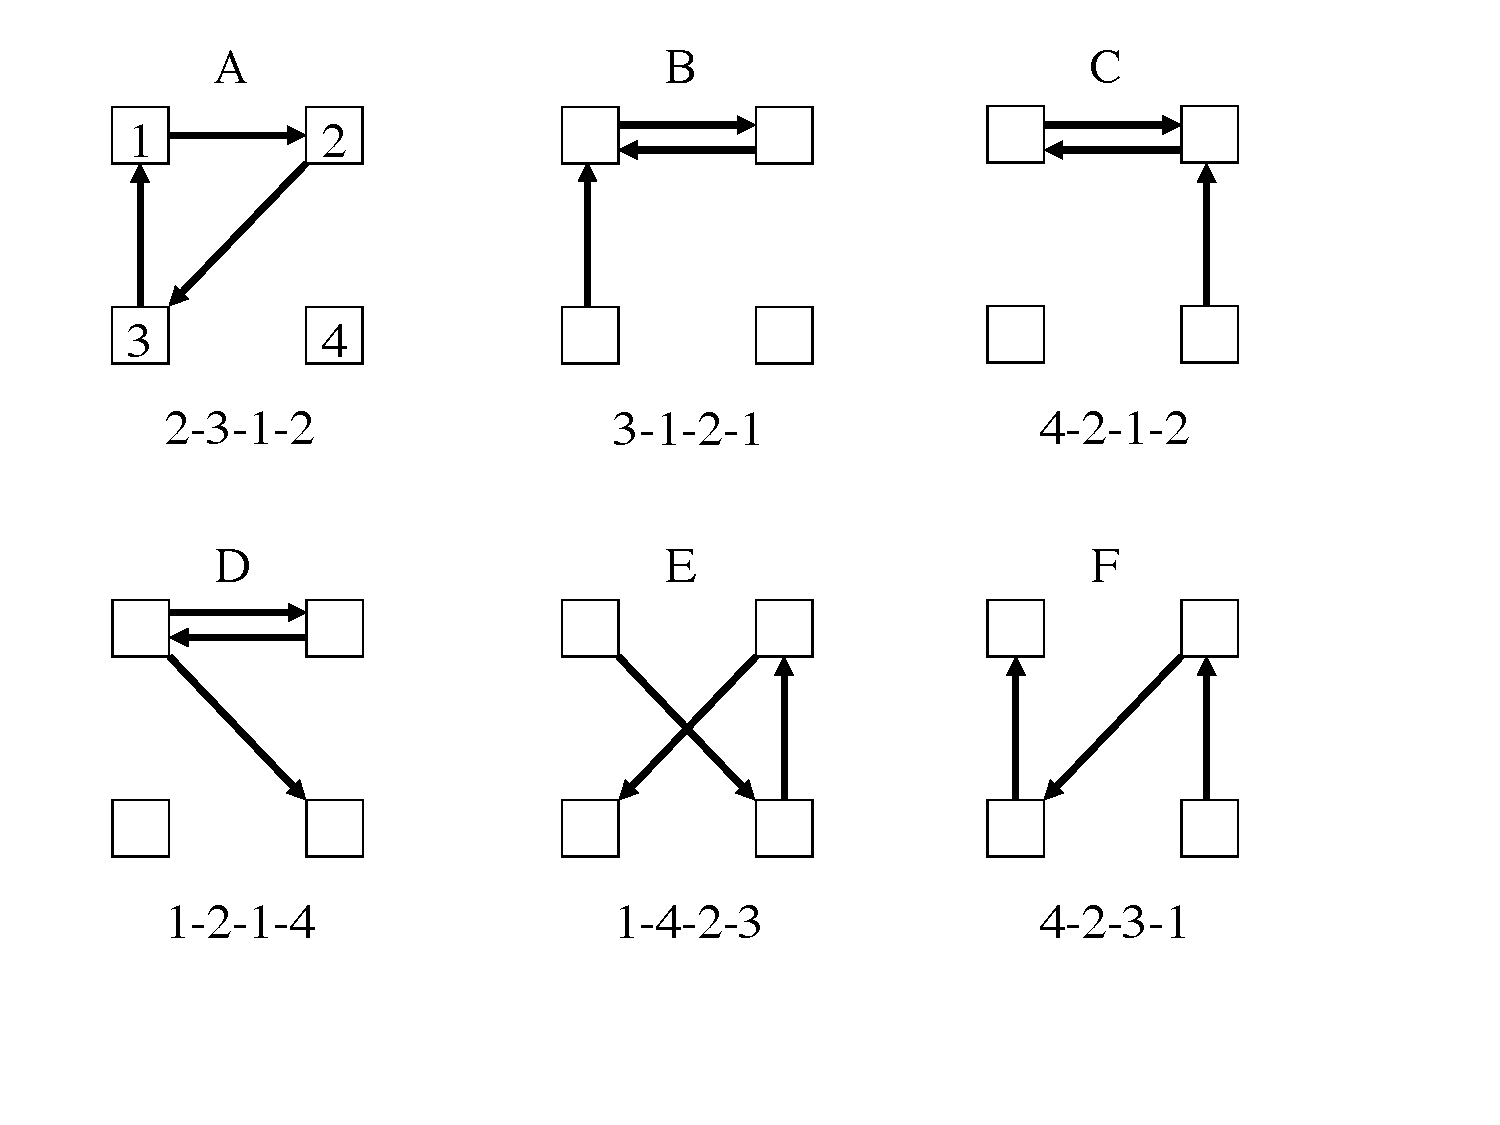
\includegraphics[width=0.48\textwidth]{figures/exp2_words}
  \caption{The six action ``word'' subsequences participants were trained on in the experiment. No position may be immediately repeated (e.g., 1-1). Words B, C, and D contain returns (e.g., 1-2-1). Words E and F contain all four locations.}
  \label{fig:exp2words}
\end{figure} 

In another experiment, Saffran \textit{et al.} investigated the effects prosodic cueing by lengthening the vowel of either the first or third (final) syllable in the word, finding that lengthening the final syllable improved performance beyond baseline or lengthening the first. Motivated by these results and the question of how reward affects learning multi-step actions, we implemented cueing in the form of different reward schemes. The rewards were aligned to the first or last action in an action sequence, analogous to the prosodic cue conditions in the Saffran \textit{et al.} study. A reward after completing a movement should emphasize the stimulus in a similar way the lengthening of a syllable does.

\subsection{Methods}

\subsubsection{Participants}

45 Leiden University students participated in exchange for 3.5 euros or one course credit. Participants were told they would receive an additional euro if they performed well (all participants were given this supplement).

\subsubsection{Procedure}

Participants were told to move the cursor as fast and accurately as possible to any target that changed to green, and that good performance could earn them a bonus euro. The stimulus display consisted of four red squares (location 1 = upper left, 2 = upper right, 3 = lower left, 4 = lower right), displayed continuously. Monitors were 17'', set to 1024 resolution, and each stimulus was 80 pixels on each side, separated by 440 pixels of white space. After arriving at the highlighted green stimulus (the other three stimuli were red), another stimulus was highlighted after a 500 ms ISI. Participants completed 4 blocks of 20 training trials, each of which contained a series of 12 locations (i.e., 3 `words'). There was a short rest break after every block. In each block, each of the 6 action `word' subsequences appeared 10 times\footnote{Note that 40 repetitions per word is far fewer than the 300 repetitions used in Saffran \textit{et al.}}, randomly distributed. Word transition frequency was not uniformly random, as no word or stimulus repetitions were allowed. Points were allocated periodically during training trials, indicated in green numbers above the arrived-at target stimulus. After training, participants were given a generating task in which they were asked to generate any action sequences they recalled from training.  In the generation task, correct predictions were rewarded (5 points per stimulus), mistakes were penalized (-20 points). After either correctly forming all words or by making 24 attempts (i.e., 72 movements) in total, participants completed the experiment. 

\subsubsection{Design}

Participants were all trained on the same sequence, but were given point rewards according to one of three different schedules, shown in Figure~\ref{fig:exp2conds}: the {\em Aligned Cue} condition awarded 15 points upon arrival at every fourth stimulus (i.e., the end of a word), the {\em Misaligned Cue} condition awarded 15 points after the first stimulus in a word, and the {\em No Cue} condition gave 5 points on arrival at every stimulus in a word but the first ({\em n.b.}: the omitted points may serve as a cue). Fifteen participants were randomly assigned to each condition.

\begin{figure}[h]
  \centering
  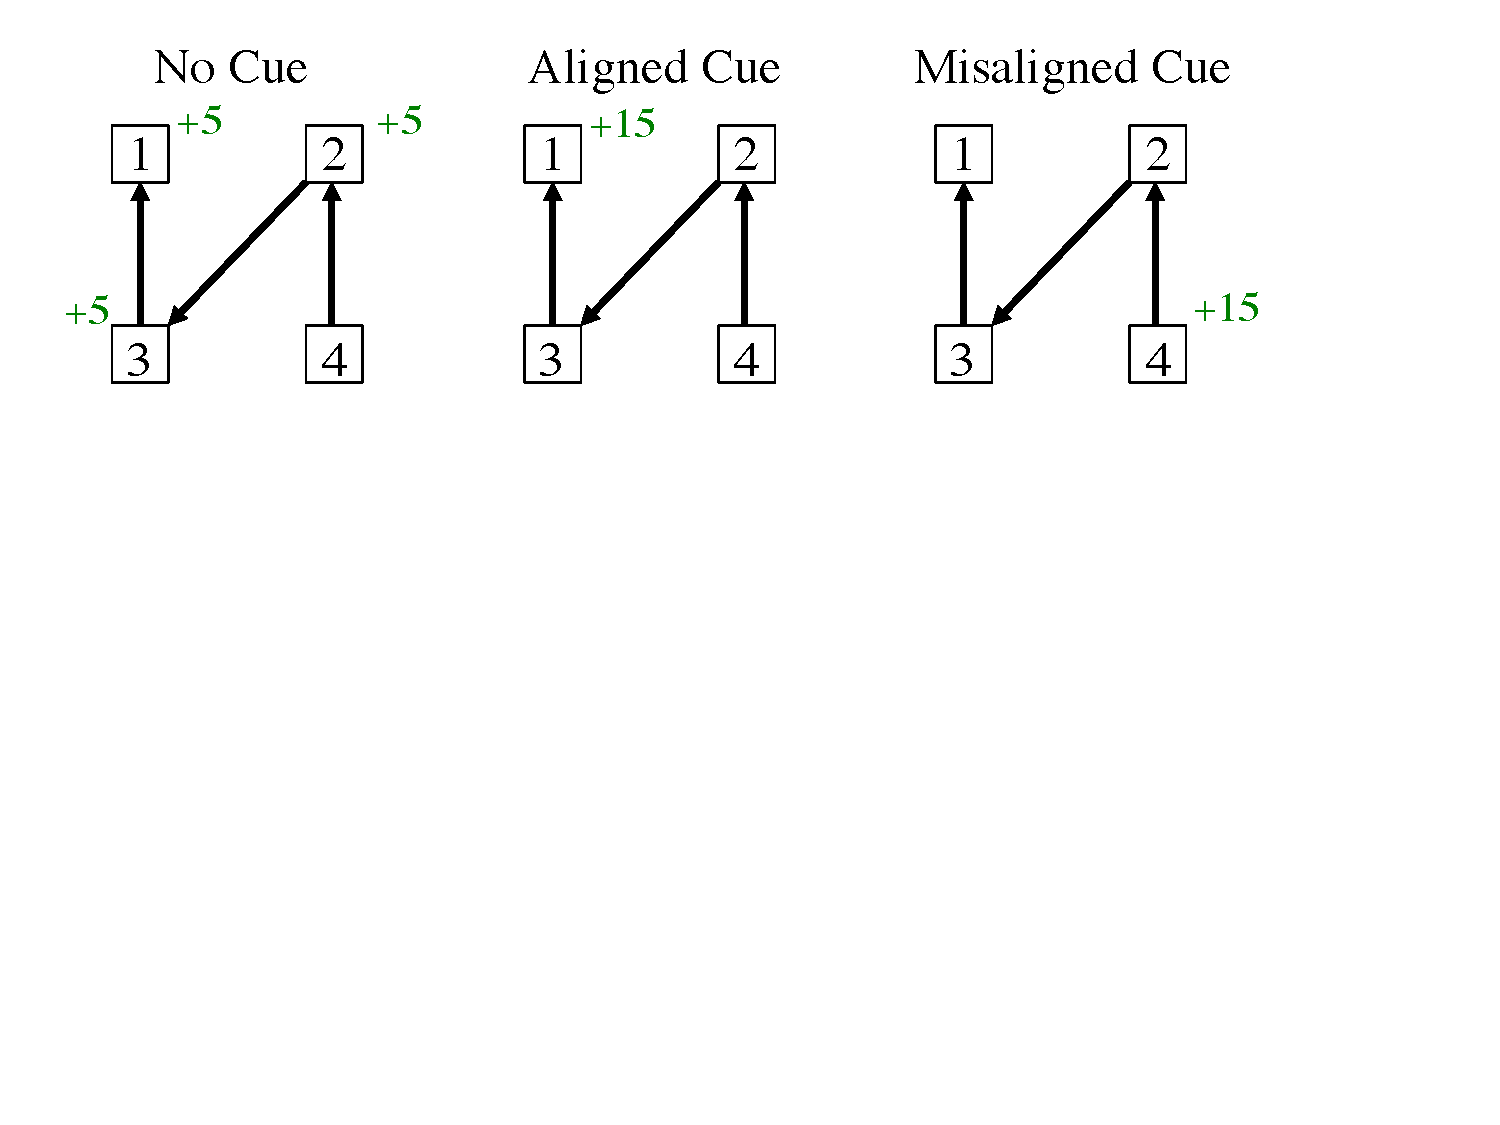
\includegraphics[width=0.48\textwidth]{figures/exp2_conditions}
  \caption{Example of the reward schedules during one word (4-2-3-1) in the three between-subjects conditions. Points were given immediately after arrival at the stimulus.}
  \label{fig:exp2conds}
\end{figure} 

\subsection{Results}

Median movement time in the training phase was 1,056 ms (sd: 1,652). Of 43,155 target arrivals, 190 were removed for being slower than 2,708 ms (median+sd). We analyzed subjects' block-by-block median movement RTs by condition and by position within the word, expecting in general that moving to the first stimulus in the next word (position 1) would be slower than within-word movements (positions 2, 3, and 4), which have higher transitional probabilities. Moreover, the different reward conditions may influence RTs at particular positions (e.g., just after the reward). A condition by position by block ($3\times4\times4$) ANCOVA showed significant main effects of block ($F$(1,42) = 29.20, $p<.001$), condition ($F$(2,42) = 5.00, $p<.001$), and position ($F$(1,42) = 16.33, $p<.001$). RT for each successive block decreased: 1127 ms, 1064 ms, 1043 ms, and 1029 ms, for blocks 1 to 4, respectively. The misaligned cue condition had the fastest overall RT (1053 ms), followed by the no cue condition (1067 ms), and the aligned condition (1077 ms)--contrary to our expectations, although further analyses will investigate within-participant speed-ups, rather than overall between condition effects. Figure~\ref{fig:exp2basic-rt} shows the mean of subjects' median RT by block for each condition, with movements between `words' (i.e., starting a new word) split out. Participants in all three conditions got faster over the course of the experiment, but no reward condition seemed to improve faster. 

\begin{figure}[h]
  \centering
  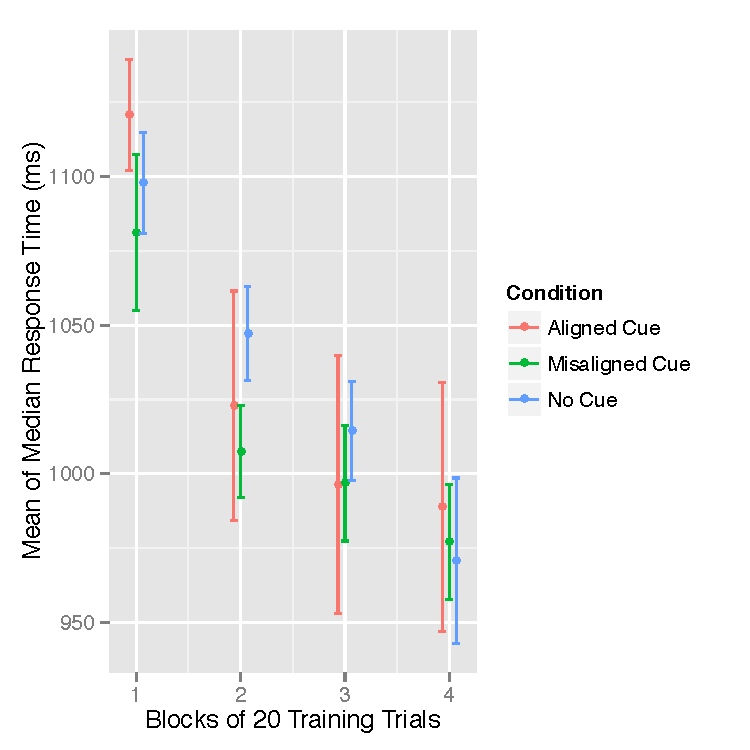
\includegraphics[width=0.48\textwidth]{figures/exp2_RT_withinWord_over_training}
  \caption{Mean of median RTs for within-word movements (i.e., not the start of a new word--position 1) for each condition by training block. Within-word movements did get faster over time, but no reward condition demonstrated a clear advantage. Error bars show +/-1SE.}
  \label{fig:exp2basic-rt}
\end{figure} 

The mean RT at within-word positions decreased until from positions 1 (i.e., the between-word movement) to 3 (1112 ms, 1074 ms, and 1026 ms, respectively), and increase again slightly at position 4 (1052 ms). This generally shows that between-word movements (moving to location 1 of a new word) are slower than within-word movements, which is quite sensible because between-word transitions are much less predictable than within-word. Finally, there was a marginally significant interaction of block and position ($F$(1,378) = 2.75, $p=.098$). Figure~\ref{fig:exp2position} shows the mean improvement, from block 1 to block 4, of subjects' median RTs for each condition by position in the subsequence. All conditions show improvements in every position, peaking at positions 3 and 4, but no condition improves much more than any other, although the misaligned cue condition trends a bit lower than the others. 

\begin{figure}[h]
  \centering
  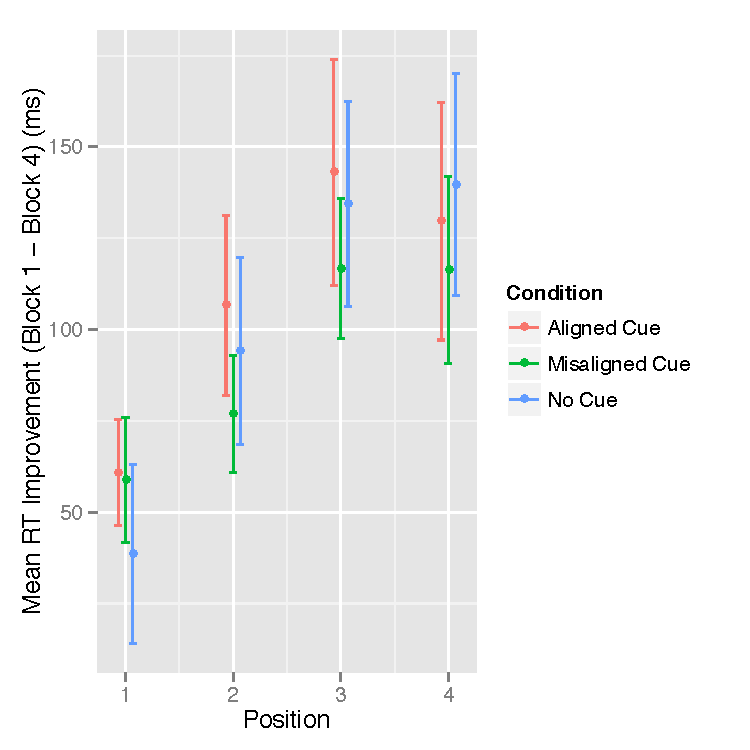
\includegraphics[width=0.48\textwidth]{figures/exp2_RTimprov_pos_by_cond}
  \caption{Mean improvement in subjects' median RTs from Block 1 to Block 4 by condition and subsequence position. Bars show +/-1SE.}
  \label{fig:exp2position}
\end{figure} 


Because the most important distinction in position is for within- vs. between-word movements, we examined the mean of each participants' RT advantage (i.e., speed-up) for within-word movements (i.e., median between-word RT minus median within-word RT) at each block, by condition. An ANCOVA showed a significant main effect of block ($F$(1,42) = 5.96, $p<.05$) and of condition ($F$(2,42) = 5.56, $p<.01$), with no significant interaction ($F$(1,172) = 0.87, $p=.42$). Shown in full in Figure~\ref{fig:exp2within_between_advantage}, after the first block the aligned cue produces a greater speed-up for within- relative to between-word movements than the other two conditions--although with variability, suggesting some learners may lag. The no cue condition looks to make a marked improvement in the final block, as well. Overall, the aligned cue condition improves within-word movements 105 ms, whereas misaligned and no cue facilitated within-word transitions 62 ms and 67 ms, respectively. Successive blocks increased the advantage, from 43 ms in block 1 to 75 ms, 84 ms, and 111 ms in blocks 2-4, respectively. In summary, although overall RTs and even mean improvements from block 1 to block 4 in within-word movements did not show a differential effect of reward schedules, looking at the within-subject advantage of within-word vs. between-word (position 1) movements showed an advantage of the aligned cue condition beyond the misaligned and no cue conditions. 

\begin{figure}[h]
  \centering
  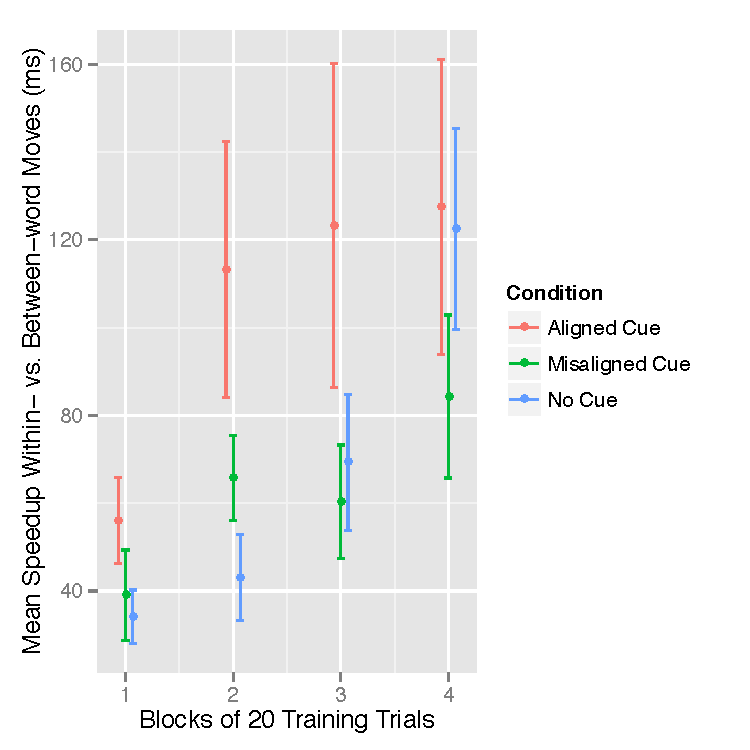
\includegraphics[width=0.48\textwidth]{figures/exp2_between_minus_withinWord_by_block}
  \caption{Mean advantage of within- vs. between-word movements from subjects' median RTs by condition across blocks. Participants in the Aligned Cue condition showed more overall speedup for the within- vs. between-word movements (with great variability), although the No Cue condition caught up in the final block. Bars show +/-1SE.}
  \label{fig:exp2within_between_advantage}
\end{figure} 

Why might we not see this reward effect in our other analyses? It may be that some words--or even particular movements--are easier to learn in some conditions, but not others: e.g., perhaps the reward in one condition highlights a particularly useful (i.e., low frequency) transition, drawing attention to it. To begin looking in more detail, we examined the mean improvement in participants' median within-word movement RTs from block 1 to block 4 for each word, by condition. Shown in Figure~\ref{fig:exp2word_improv}, unsurprisingly participants in all conditions improve at all six action subsequences. However, one word stood out as more difficult: subsequence 1-4-2-3 saw the least improvement in all three conditions, and was lowest of all in the aligned cue condition. We do not yet have a hypothesis about why this should be so, but we believe it warrants further investigation. Of the other five words, only 3-1-2-1 stood out as being a bit easier in the no cue condition, but for no readily apparent reason. 

We examined the RT improvements from block 1 to block 4 for each the six single within-word movements (e.g., 2-1, in word B, C, and D) by condition, to see if the reward schedules may be motivating participants to learn more (or simply move faster) for during particular parts of the sequence. Shown in Figure~\ref{fig:exp2move_improv}, the smallest improvement is seen in movements 1-4 and 2-3 in the aligned cue condition: the two diagonal components of the standout slow word (1-4-2-3) for that condition. Overall, the misaligned cue showed consistent improvement in all of the movements, while the other two conditions showed improvements for particular movements. 

\begin{figure}[h]
  \centering
  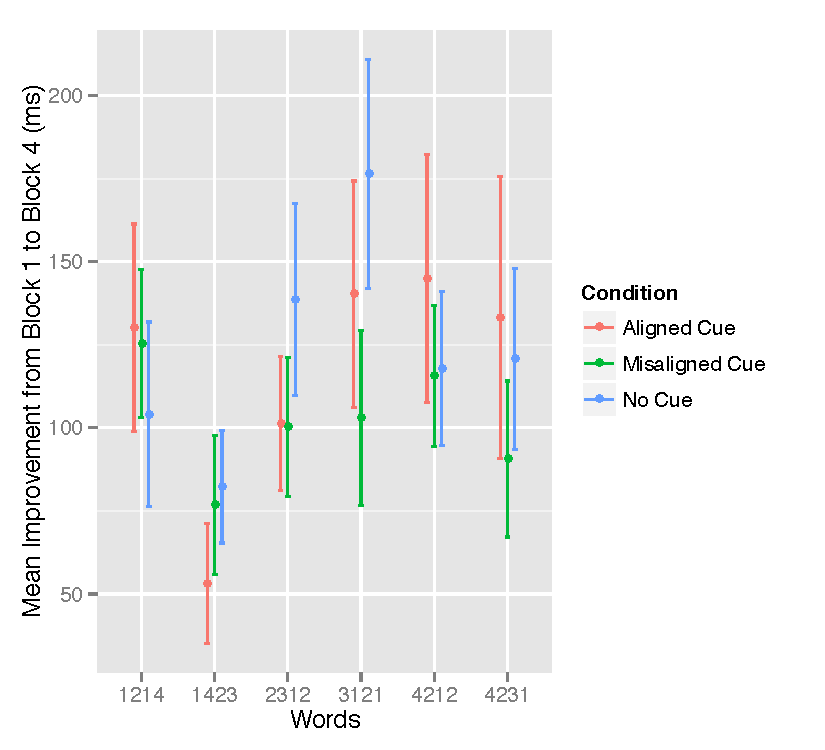
\includegraphics[width=0.48\textwidth]{figures/exp2_withinWordRT_improve_by_cond}
  \caption{Mean improvement in subjects' median within-word movement RTs from block 1 to block 4 for each word, by condition. Bars show +/-1SE.}
  \label{fig:exp2word_improv}
\end{figure} 


\begin{figure}[h]
  \centering
  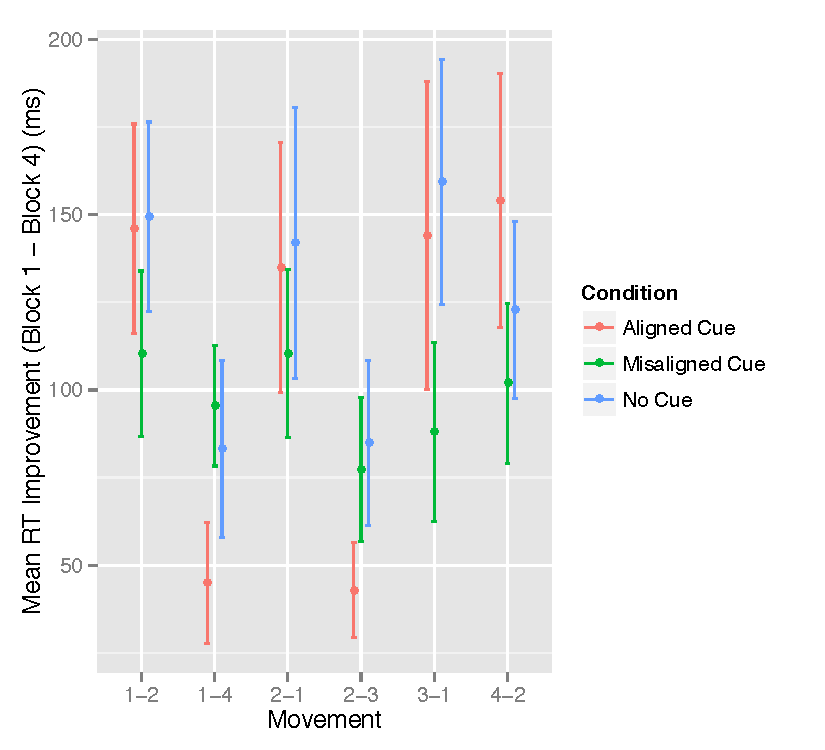
\includegraphics[width=0.48\textwidth]{figures/exp2_RTimprov_movement_by_cond}
  \caption{Mean improvement in subjects' median RTs from block 1 to block 4 for each within-word movement, by condition. Bars show +/-1SE.}
  \label{fig:exp2move_improv}
\end{figure} 

\begin{figure}[h]
  \centering
  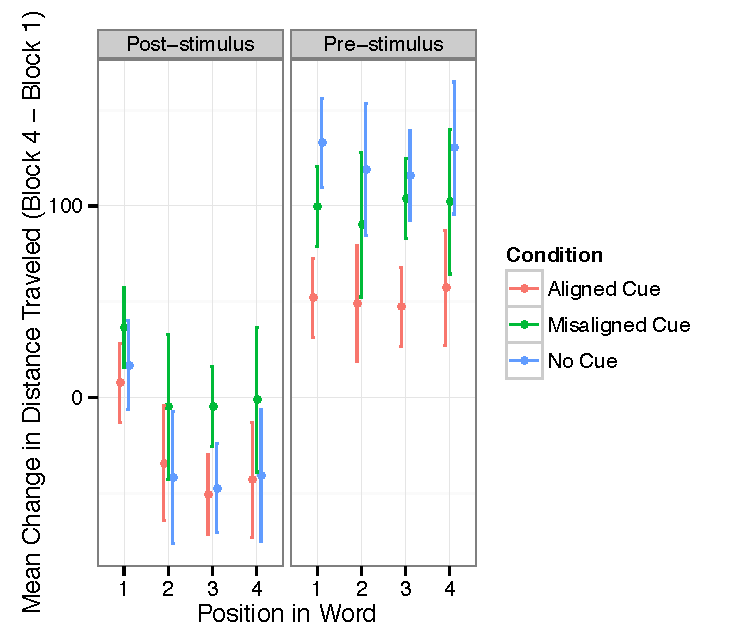
\includegraphics[width=0.49\textwidth]{figures/exp2_change_in_distance_by_position_b1_to_b4} 
  \caption{The mean change in distance (pixels) traveled from Block 1 to Block 4 after the next stimulus appears (post-stimulus) compared to the 500 ms pre-stimulus period, when predictive movements may be made. More distance was covered during the pre-stimulus portion of each movement for all conditions--and equally at all within-word positions--although, the Aligned Cue condition shows less predictive motion. The post-stimulus portion of movements show a decrease in distance traveled for all but the the first position, although the Misaligned Cue condition shows little change.}
  \label{fig:predictive}
\end{figure} 

Accuracy during training was not analyzed as subjects only needed to move the cursor to the highlighted target, a somewhat trivial task with an error rate of less than 1\%. However, the mouse movement trajectories made during training--and their dynamics over the course of training--are of great interest and complexity. Figure~\ref{fig:predictive} shows the mean change in the total distance traveled (block 4 - 1) during the first 500 ms of each movement, before the next stimulus has been shown, compared to the post-stimulus portion of the movement, split by condition and position within the action word. At all word positions a greater distance is traveled in the pre-stimulus predictive portion of the movement by the end of training, although the Aligned Cue condition shows less predictive motion than the other conditions. Less distance is traveled for all but the first position (when there is greater uncertainty) during the post-stimulus portion, showing that subjects were moving appropriately. Moreover, an ANOVA of  the number of cursor positions spent outside the stimulus boxes during the predictive (i.e., ISI) period showed a significant main effect of training half ($F$(1,44) = 4.05, $p<.05$), but no significant main effect of condition ($F$(2,80) = 2.22, $p=.11$), nor a significant interaction ($F$(2,80) = 0.79, $p=.46$). As suggested by Figure~\ref{fig:predictive}, participants spent more of the predictive ISI in-between stimuli in the late half of training, a mean of 15,266 points in the second half vs. 14,397 points in the first half. Thus, the decreased inter-stimulus arrival times observed across training are not necessarily only a speedup of movement, but are enabled by earlier, predictive movement toward the next stimulus.


Overall performance in the generation task was quite low and did not differ by reward condition: of 24 attempts per subject, a mean of only 8.5 words were reproduced in the aligned and misaligned cue conditions, compared to 9.5 in the no cue condition. This indicates that subjects did not gain much explicit knowledge of the studied sequences.

\section{General Discussion}

In the present study we used a trajectory-tracking adaptation of the serial reaction time task to investigate the learning of action `words' (i.e., subsequences three movements long), inspired by the design of a statistical word segmentation study \cite{Saffran:1996}. Participants were given a long sequence of stimuli to direct their cursor to, and we observed reaction times decrease within-word as they learned the regular subsequences. Between-word movements did not show as much speed-up. In principle, this replicates the Saffran \textit{et al.} \cite{Saffran:1996} finding that a continuous stream of syllables (in our case, movements) can be segmented into interchangeable words (i.e., action subsequences) solely on the basis of between- vs. within-word transition probabilities. By recording responses during training, we were able to see learning online, instead of only with a final test.

Furthermore, we manipulated reward schedules--giving learners a lump sum of points after completing each word, after the first movement in a word, or points spread across the movements in a word--in an attempt to help or hinder learning, as in prosodic cueing studies of word segmentation \cite{Saffran:1996}. Fu \textit{et al.} \cite{Fu:2008} found that offering a reward to participants in an SRT task increased motivation, resulting in higher generation task performance. Although our reward manipulation had surprisingly little effect on the rate or magnitude of subsequence learning during training, we did find that within-word movements sped up more relative to between-word movements in the aligned cue condition than in the misaligned or no cue conditions. Our analysis of predictive movements, made before the next stimulus appeared, showed that people made more of these movements in the late half of training than early in training. However, no differences were found between conditions. Further in-depth analyses of particular motions (e.g., in terms of their relative frequency and predictability) and average response trajectories may yet reveal more subtle effects of reward on learning.

Our study acknowledges that complex actions are rarely completely unambiguous, but rather often have probabilistic dependencies on the past stimuli and actions. We wanted to investigate how people learn sequences that have statistical uncertainty at different levels: the next action may be ambiguous given only the previous stimulus (e.g., 1-2 occurs in four words), but may be less ambiguous conditioned on the previous two stimuli (3-1-2 occurs only twice). This is similar to the motivations espoused by statistical learning researchers (e.g., \cite{Saffran:1996}). Indeed, implicit learning and statistical learning research often have the same motivations and intuitions, and should be more strongly linked \cite{Perruchet:2006}. The trajectory SRT paradigm is suitable for building this bridge--and of a material that supports detailed analyses, which promise to reveal the continuous dynamics of the underyling cognitive processes \cite{Spivey:2006,Kachergis:2011g}.

In future work, we plan to include more detailed analyses of movement times and trajectories as a function of transitional probabilities and overall probability of occurrence. Sequential action, in all its complexity, is the foundation of most human pursuits, and it is thus important to understand how people learn these sequences. We posit that the best way to measure this learning is to measure actual movement responses, and we hope that researchers from diverse backgrounds will join us. This approach will not only yield a better understanding of how humans learn, but can help us create more adaptive robot systems that we will one day work alongside (for a review, see \cite{deKleijn:2014}).


\section*{Acknowledgment}

The preparation of this work was supported by the European Commission (EU Cognitive Systems project ROBOHOW.COG; FP7-ICT-2011).


\bibliographystyle{IEEEtran}

\bibliography{SRT_trajectory_refs}

\end{document}
